\documentclass[twoside]{article}

% Packages required by doxygen
\usepackage{fixltx2e}
\usepackage{calc}
\usepackage{doxygen}
\usepackage[export]{adjustbox} % also loads graphicx
\usepackage{graphicx}
\usepackage[utf8]{inputenc}
\usepackage{makeidx}
\usepackage{multicol}
\usepackage{multirow}
\PassOptionsToPackage{warn}{textcomp}
\usepackage{textcomp}
\usepackage[nointegrals]{wasysym}
\usepackage[table]{xcolor}

% Font selection
\usepackage[T1]{fontenc}
\usepackage[scaled=.90]{helvet}
\usepackage{courier}
\usepackage{amssymb}
\usepackage{sectsty}
\renewcommand{\familydefault}{\sfdefault}
\allsectionsfont{%
  \fontseries{bc}\selectfont%
  \color{darkgray}%
}
\renewcommand{\DoxyLabelFont}{%
  \fontseries{bc}\selectfont%
  \color{darkgray}%
}
\newcommand{\+}{\discretionary{\mbox{\scriptsize$\hookleftarrow$}}{}{}}

% Page & text layout
\usepackage{geometry}
\geometry{%
  a4paper,%
  top=2.5cm,%
  bottom=2.5cm,%
  left=2.5cm,%
  right=2.5cm%
}
\tolerance=750
\hfuzz=15pt
\hbadness=750
\setlength{\emergencystretch}{15pt}
\setlength{\parindent}{0cm}
\setlength{\parskip}{3ex plus 2ex minus 2ex}
\makeatletter
\renewcommand{\paragraph}{%
  \@startsection{paragraph}{4}{0ex}{-1.0ex}{1.0ex}{%
    \normalfont\normalsize\bfseries\SS@parafont%
  }%
}
\renewcommand{\subparagraph}{%
  \@startsection{subparagraph}{5}{0ex}{-1.0ex}{1.0ex}{%
    \normalfont\normalsize\bfseries\SS@subparafont%
  }%
}
\makeatother

% Headers & footers
\usepackage{fancyhdr}
\pagestyle{fancyplain}
\fancyhead[LE]{\fancyplain{}{\bfseries\thepage}}
\fancyhead[CE]{\fancyplain{}{}}
\fancyhead[RE]{\fancyplain{}{\bfseries\leftmark}}
\fancyhead[LO]{\fancyplain{}{\bfseries\rightmark}}
\fancyhead[CO]{\fancyplain{}{}}
\fancyhead[RO]{\fancyplain{}{\bfseries\thepage}}
\fancyfoot[LE]{\fancyplain{}{}}
\fancyfoot[CE]{\fancyplain{}{}}
\fancyfoot[RE]{\fancyplain{}{\bfseries\scriptsize Generated by Doxygen }}
\fancyfoot[LO]{\fancyplain{}{\bfseries\scriptsize Generated by Doxygen }}
\fancyfoot[CO]{\fancyplain{}{}}
\fancyfoot[RO]{\fancyplain{}{}}
\renewcommand{\footrulewidth}{0.4pt}
\renewcommand{\sectionmark}[1]{%
  \markright{\thesection\ #1}%
}

% Indices & bibliography
\usepackage{natbib}
\usepackage[titles]{tocloft}
\setcounter{tocdepth}{3}
\setcounter{secnumdepth}{5}
\makeindex

% Hyperlinks (required, but should be loaded last)
\usepackage{ifpdf}
\ifpdf
  \usepackage[pdftex,pagebackref=true]{hyperref}
\else
  \usepackage[ps2pdf,pagebackref=true]{hyperref}
\fi
\hypersetup{%
  colorlinks=true,%
  linkcolor=blue,%
  citecolor=blue,%
  unicode%
}

% Custom commands
\newcommand{\clearemptydoublepage}{%
  \newpage{\pagestyle{empty}\cleardoublepage}%
}

\usepackage{caption}
\captionsetup{labelsep=space,justification=centering,font={bf},singlelinecheck=off,skip=4pt,position=top}

%===== C O N T E N T S =====

\begin{document}

% Titlepage & ToC
\hypersetup{pageanchor=false,
             bookmarksnumbered=true,
             pdfencoding=unicode
            }
\pagenumbering{roman}
\begin{titlepage}
\vspace*{7cm}
\begin{center}%
{\Large Manual inheritance and membership }\\
\vspace*{1cm}
{\large Generated by Doxygen 1.8.11}\\
\end{center}
\end{titlepage}
\tableofcontents
\pagenumbering{arabic}
\hypersetup{pageanchor=true}

%--- Begin generated contents ---
\section{Class Documentation}
\hypertarget{struct_car}{}\subsection{Car Struct Reference}
\label{struct_car}\index{Car@{Car}}


\hyperlink{struct_car}{Car} type.  


Inheritance diagram for Car\+:\begin{figure}[H]
\begin{center}
\leavevmode
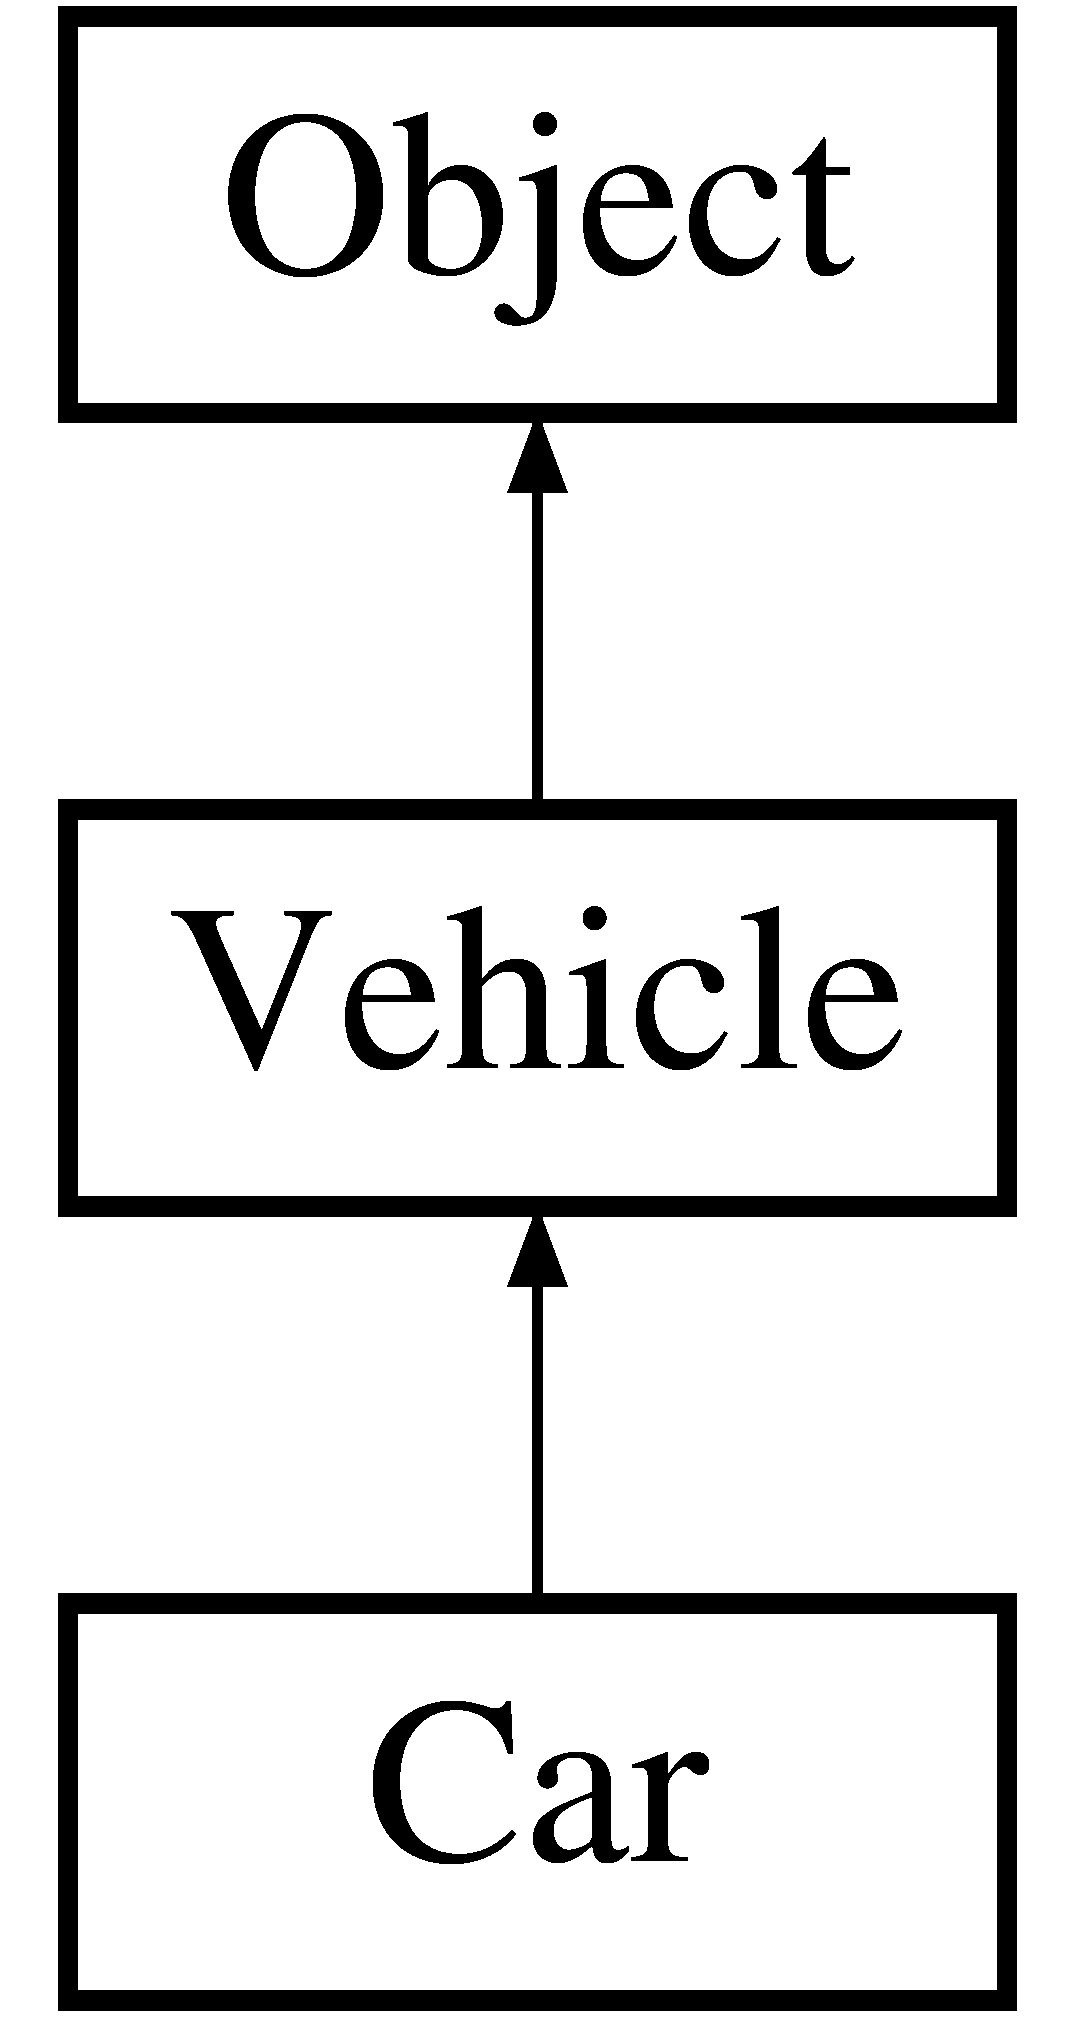
\includegraphics[height=3.000000cm]{struct_car}
\end{center}
\end{figure}
\subsubsection*{Protected Attributes}
\begin{DoxyCompactItemize}
\item 
\hyperlink{struct_vehicle}{Vehicle} \hyperlink{struct_car_ab8ff28306286da5a8b14fa9bdccaafaa}{base}\hypertarget{struct_car_ab8ff28306286da5a8b14fa9bdccaafaa}{}\label{struct_car_ab8ff28306286da5a8b14fa9bdccaafaa}

\begin{DoxyCompactList}\small\item\em Base class. \end{DoxyCompactList}\end{DoxyCompactItemize}
\subsubsection*{Additional Inherited Members}


\subsubsection{Detailed Description}
\hyperlink{struct_car}{Car} type. 

\hyperlink{struct_car}{Car} class. 

The documentation for this struct was generated from the following file\+:\begin{DoxyCompactItemize}
\item 
\hyperlink{manual_8c}{manual.\+c}\end{DoxyCompactItemize}

\hypertarget{struct_object}{}\subsection{Object Struct Reference}
\label{struct_object}\index{Object@{Object}}


\hyperlink{struct_object}{Object} type.  


Inheritance diagram for Object\+:\begin{figure}[H]
\begin{center}
\leavevmode
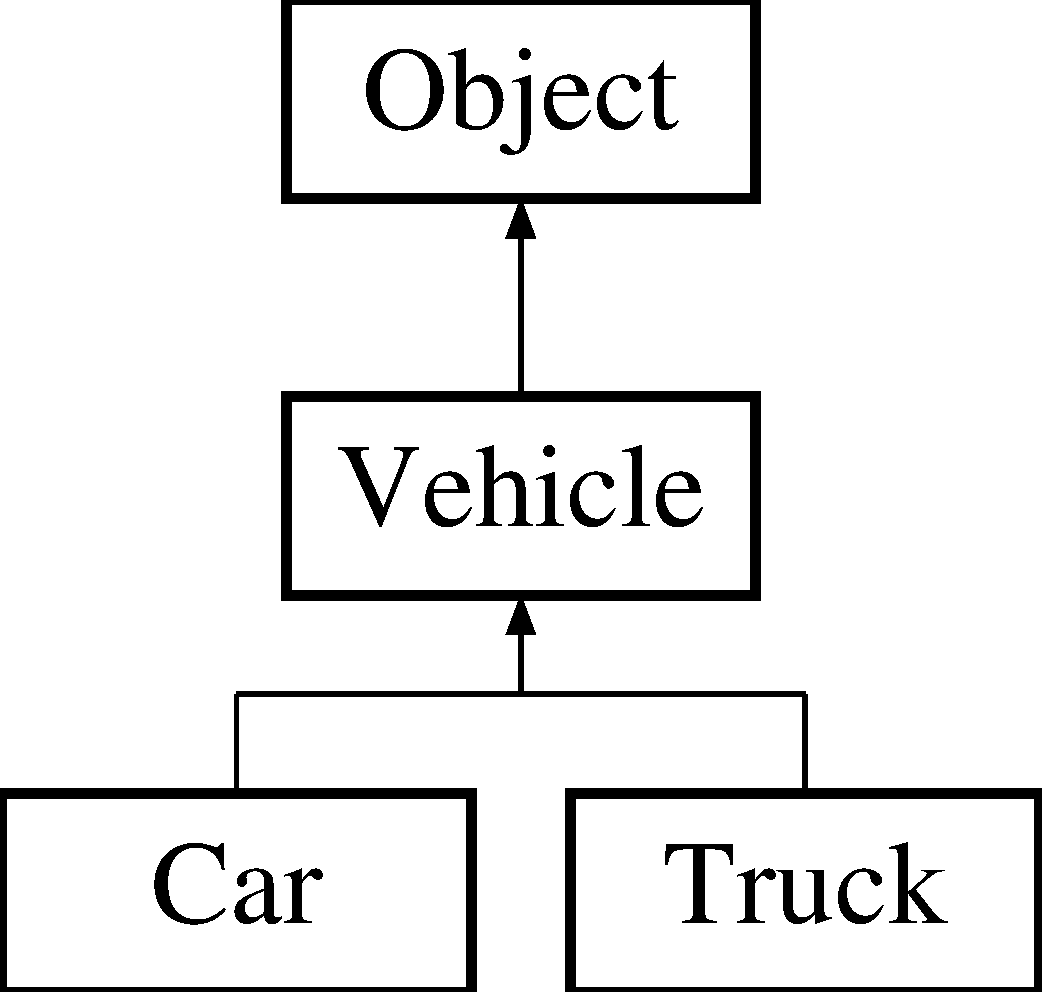
\includegraphics[height=3.000000cm]{struct_object}
\end{center}
\end{figure}
\subsubsection*{Public Member Functions}
\begin{DoxyCompactItemize}
\item 
static \hyperlink{struct_object}{Object} $\ast$ \hyperlink{struct_object_a71225073d06a793b9a6ea9263ed37b12}{obj\+Ref} (\hyperlink{struct_object}{Object} $\ast$obj)
\item 
static \hyperlink{struct_object}{Object} $\ast$ \hyperlink{struct_object_a924ee0cecc906d148022b3f0d6325cfb}{obj\+Unref} (\hyperlink{struct_object}{Object} $\ast$obj)
\end{DoxyCompactItemize}
\subsubsection*{Private Attributes}
\begin{DoxyCompactItemize}
\item 
int \hyperlink{struct_object_a1b6037fba835e83243ababce426ff9af}{ref}\hypertarget{struct_object_a1b6037fba835e83243ababce426ff9af}{}\label{struct_object_a1b6037fba835e83243ababce426ff9af}

\begin{DoxyCompactList}\small\item\em Reference count. \end{DoxyCompactList}\end{DoxyCompactItemize}


\subsubsection{Detailed Description}
\hyperlink{struct_object}{Object} type. 

Base object class. 

\subsubsection{Member Function Documentation}
\index{Object@{Object}!obj\+Ref@{obj\+Ref}}
\index{obj\+Ref@{obj\+Ref}!Object@{Object}}
\paragraph[{\texorpdfstring{obj\+Ref(\+Object $\ast$obj)}{objRef(Object *obj)}}]{\setlength{\rightskip}{0pt plus 5cm}static {\bf Object} $\ast$ obj\+Ref (
\begin{DoxyParamCaption}
\item[{{\bf Object} $\ast$}]{obj}
\end{DoxyParamCaption}
)}\hypertarget{struct_object_a71225073d06a793b9a6ea9263ed37b12}{}\label{struct_object_a71225073d06a793b9a6ea9263ed37b12}
Increments object reference count by one. \index{Object@{Object}!obj\+Unref@{obj\+Unref}}
\index{obj\+Unref@{obj\+Unref}!Object@{Object}}
\paragraph[{\texorpdfstring{obj\+Unref(\+Object $\ast$obj)}{objUnref(Object *obj)}}]{\setlength{\rightskip}{0pt plus 5cm}static {\bf Object} $\ast$ obj\+Unref (
\begin{DoxyParamCaption}
\item[{{\bf Object} $\ast$}]{obj}
\end{DoxyParamCaption}
)}\hypertarget{struct_object_a924ee0cecc906d148022b3f0d6325cfb}{}\label{struct_object_a924ee0cecc906d148022b3f0d6325cfb}
Decrements object reference count by one. 

The documentation for this struct was generated from the following file\+:\begin{DoxyCompactItemize}
\item 
\hyperlink{manual_8c}{manual.\+c}\end{DoxyCompactItemize}

\hypertarget{struct_truck}{}\subsection{Truck Struct Reference}
\label{struct_truck}\index{Truck@{Truck}}


\hyperlink{struct_truck}{Truck} type.  


Inheritance diagram for Truck\+:\begin{figure}[H]
\begin{center}
\leavevmode
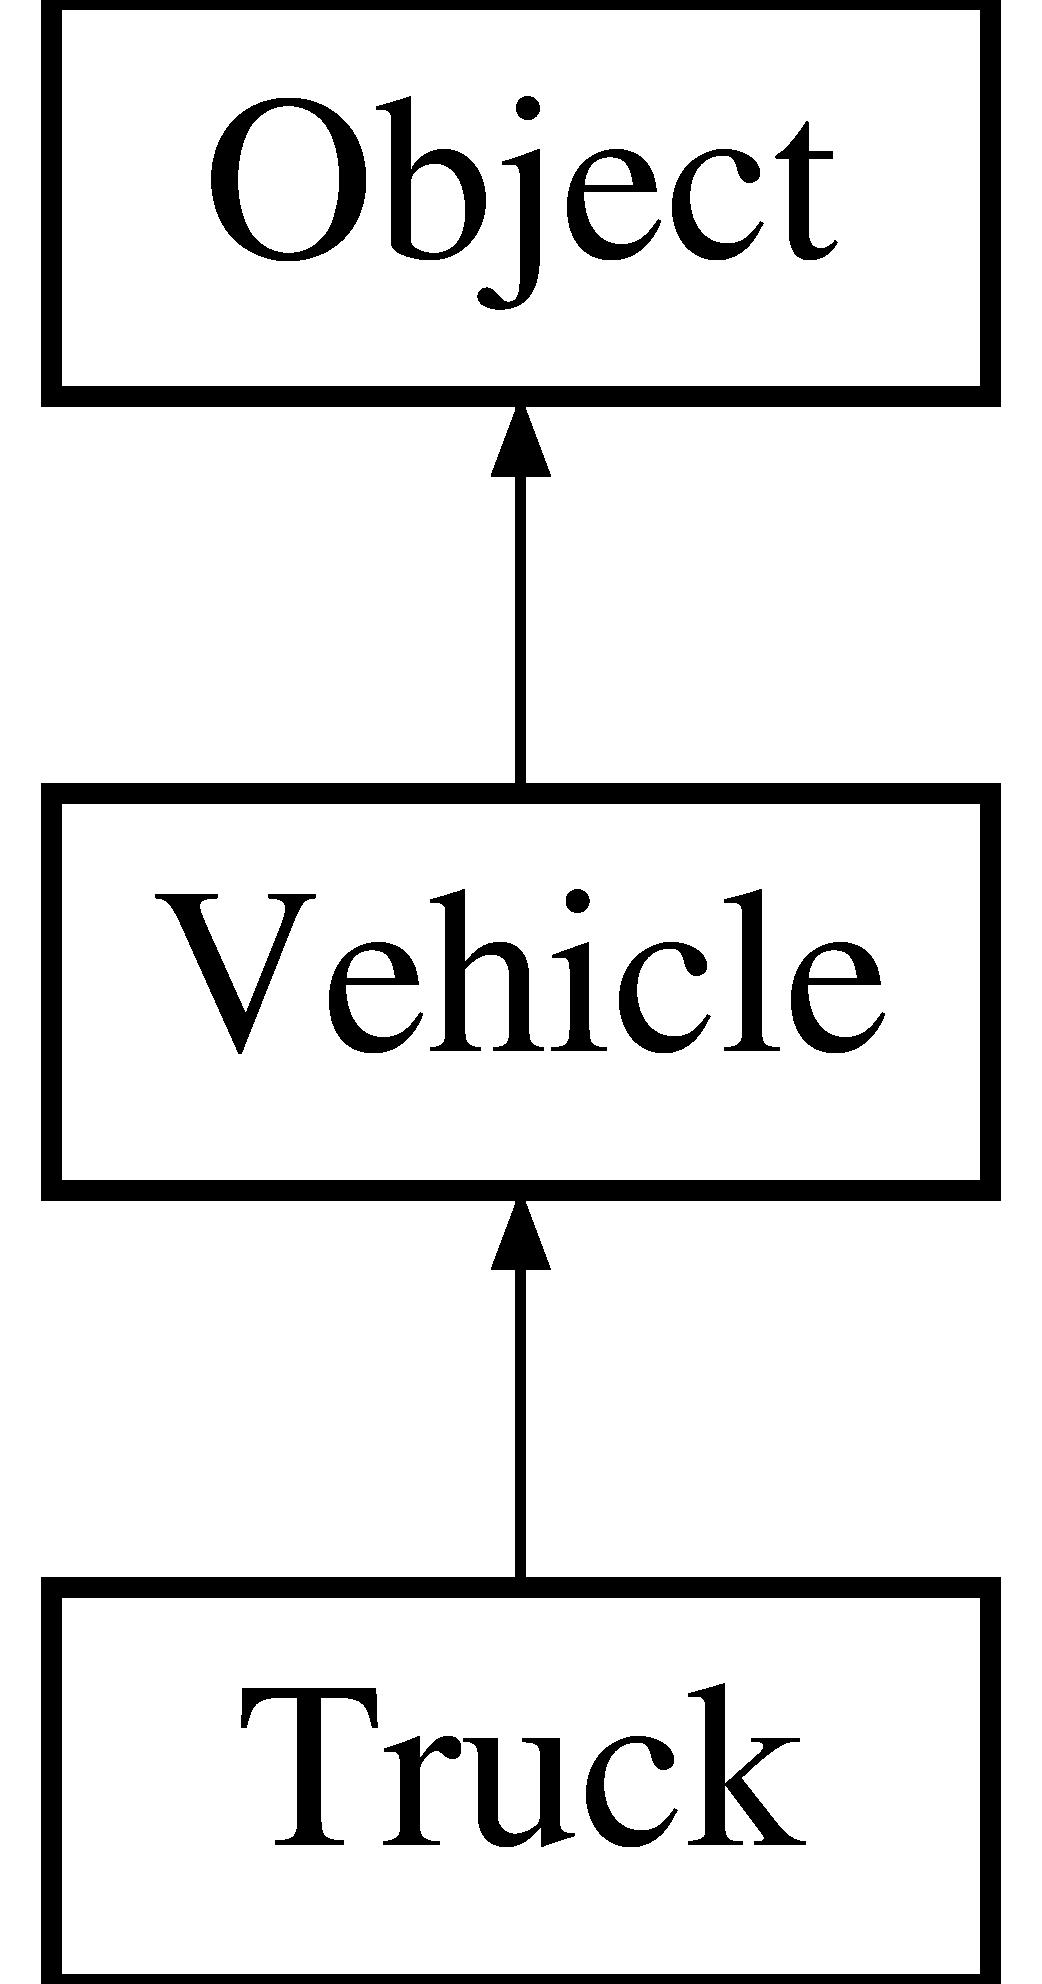
\includegraphics[height=3.000000cm]{struct_truck}
\end{center}
\end{figure}
\subsubsection*{Protected Attributes}
\begin{DoxyCompactItemize}
\item 
\hyperlink{struct_vehicle}{Vehicle} \hyperlink{struct_truck_ad0ac321609dda1a6c552488b05ec7ac8}{base}\hypertarget{struct_truck_ad0ac321609dda1a6c552488b05ec7ac8}{}\label{struct_truck_ad0ac321609dda1a6c552488b05ec7ac8}

\begin{DoxyCompactList}\small\item\em Base class. \end{DoxyCompactList}\end{DoxyCompactItemize}
\subsubsection*{Additional Inherited Members}


\subsubsection{Detailed Description}
\hyperlink{struct_truck}{Truck} type. 

\hyperlink{struct_truck}{Truck} class. 

The documentation for this struct was generated from the following file\+:\begin{DoxyCompactItemize}
\item 
\hyperlink{manual_8c}{manual.\+c}\end{DoxyCompactItemize}

\hypertarget{struct_vehicle}{}\subsection{Vehicle Struct Reference}
\label{struct_vehicle}\index{Vehicle@{Vehicle}}


\hyperlink{struct_vehicle}{Vehicle} type.  


Inheritance diagram for Vehicle\+:\begin{figure}[H]
\begin{center}
\leavevmode
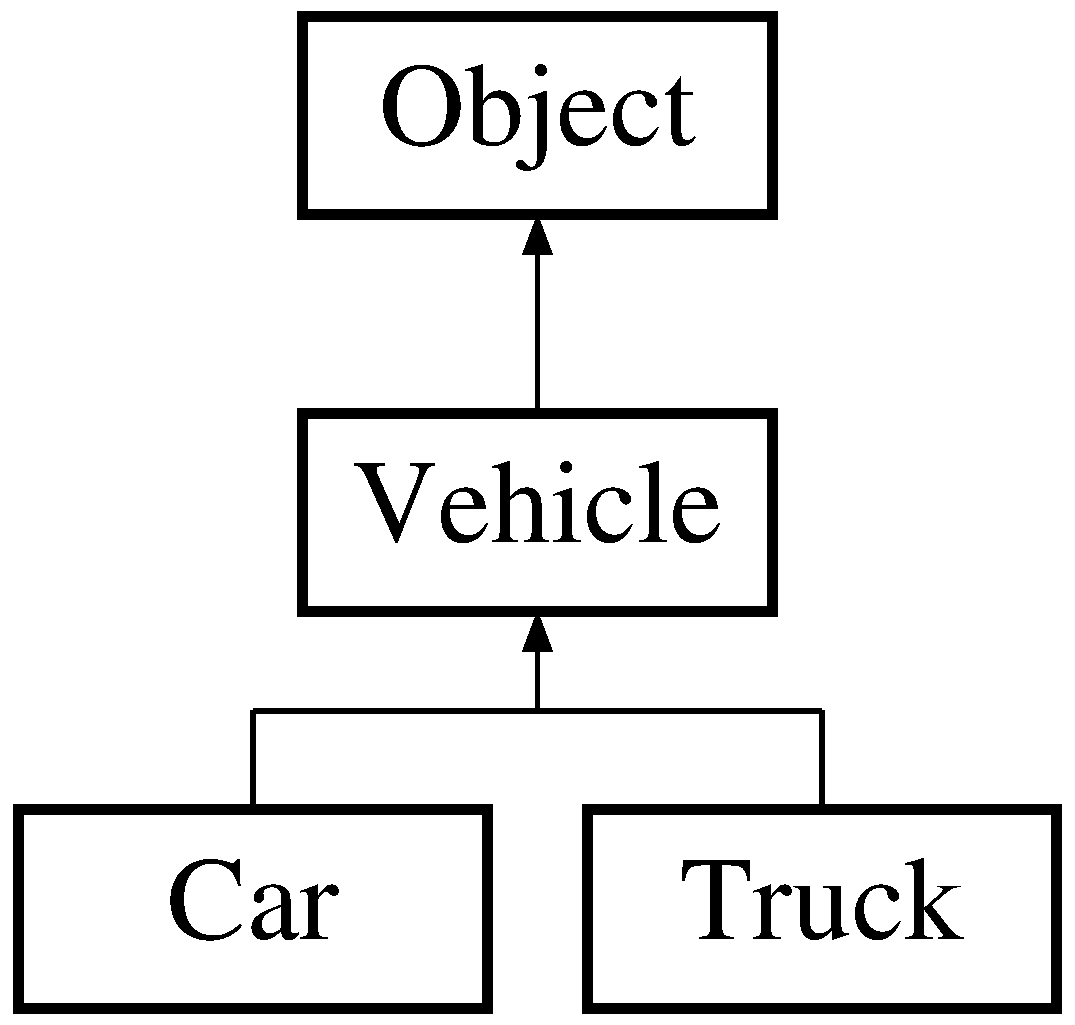
\includegraphics[height=3.000000cm]{struct_vehicle}
\end{center}
\end{figure}
\subsubsection*{Public Member Functions}
\begin{DoxyCompactItemize}
\item 
void \hyperlink{struct_vehicle_a6891d3d28853bc3fdd075596dc6de9f8}{vehicle\+Start} (\hyperlink{struct_vehicle}{Vehicle} $\ast$obj)
\item 
void \hyperlink{struct_vehicle_a4dcbcba43792dcd673a552b14479ab77}{vehicle\+Stop} (\hyperlink{struct_vehicle}{Vehicle} $\ast$obj)
\end{DoxyCompactItemize}
\subsubsection*{Protected Attributes}
\begin{DoxyCompactItemize}
\item 
\hyperlink{struct_object}{Object} \hyperlink{struct_vehicle_ad7970f528d429f6fc1725173e93a77c2}{base}\hypertarget{struct_vehicle_ad7970f528d429f6fc1725173e93a77c2}{}\label{struct_vehicle_ad7970f528d429f6fc1725173e93a77c2}

\begin{DoxyCompactList}\small\item\em Base class. \end{DoxyCompactList}\end{DoxyCompactItemize}


\subsubsection{Detailed Description}
\hyperlink{struct_vehicle}{Vehicle} type. 

\hyperlink{struct_vehicle}{Vehicle} class. 

\subsubsection{Member Function Documentation}
\index{Vehicle@{Vehicle}!vehicle\+Start@{vehicle\+Start}}
\index{vehicle\+Start@{vehicle\+Start}!Vehicle@{Vehicle}}
\paragraph[{\texorpdfstring{vehicle\+Start(\+Vehicle $\ast$obj)}{vehicleStart(Vehicle *obj)}}]{\setlength{\rightskip}{0pt plus 5cm}void vehicle\+Start (
\begin{DoxyParamCaption}
\item[{{\bf Vehicle} $\ast$}]{obj}
\end{DoxyParamCaption}
)}\hypertarget{struct_vehicle_a6891d3d28853bc3fdd075596dc6de9f8}{}\label{struct_vehicle_a6891d3d28853bc3fdd075596dc6de9f8}
Starts the vehicle. \index{Vehicle@{Vehicle}!vehicle\+Stop@{vehicle\+Stop}}
\index{vehicle\+Stop@{vehicle\+Stop}!Vehicle@{Vehicle}}
\paragraph[{\texorpdfstring{vehicle\+Stop(\+Vehicle $\ast$obj)}{vehicleStop(Vehicle *obj)}}]{\setlength{\rightskip}{0pt plus 5cm}void vehicle\+Stop (
\begin{DoxyParamCaption}
\item[{{\bf Vehicle} $\ast$}]{obj}
\end{DoxyParamCaption}
)}\hypertarget{struct_vehicle_a4dcbcba43792dcd673a552b14479ab77}{}\label{struct_vehicle_a4dcbcba43792dcd673a552b14479ab77}
Stops the vehicle. 

The documentation for this struct was generated from the following file\+:\begin{DoxyCompactItemize}
\item 
\hyperlink{manual_8c}{manual.\+c}\end{DoxyCompactItemize}

\section{File Documentation}
\hypertarget{manual_8c}{}\subsection{manual.\+c File Reference}
\label{manual_8c}\index{manual.\+c@{manual.\+c}}
\subsubsection*{Classes}
\begin{DoxyCompactItemize}
\item 
struct \hyperlink{struct_object}{Object}
\begin{DoxyCompactList}\small\item\em \hyperlink{struct_object}{Object} type. \end{DoxyCompactList}\item 
struct \hyperlink{struct_vehicle}{Vehicle}
\begin{DoxyCompactList}\small\item\em \hyperlink{struct_vehicle}{Vehicle} type. \end{DoxyCompactList}\item 
struct \hyperlink{struct_car}{Car}
\begin{DoxyCompactList}\small\item\em \hyperlink{struct_car}{Car} type. \end{DoxyCompactList}\item 
struct \hyperlink{struct_truck}{Truck}
\begin{DoxyCompactList}\small\item\em \hyperlink{struct_truck}{Truck} type. \end{DoxyCompactList}\end{DoxyCompactItemize}
\subsubsection*{Functions}
\begin{DoxyCompactItemize}
\item 
int \hyperlink{manual_8c_a840291bc02cba5474a4cb46a9b9566fe}{main} (void)
\end{DoxyCompactItemize}


\subsubsection{Function Documentation}
\index{manual.\+c@{manual.\+c}!main@{main}}
\index{main@{main}!manual.\+c@{manual.\+c}}
\paragraph[{\texorpdfstring{main(void)}{main(void)}}]{\setlength{\rightskip}{0pt plus 5cm}int main (
\begin{DoxyParamCaption}
\item[{void}]{}
\end{DoxyParamCaption}
)}\hypertarget{manual_8c_a840291bc02cba5474a4cb46a9b9566fe}{}\label{manual_8c_a840291bc02cba5474a4cb46a9b9566fe}
Main function.

Ref \hyperlink{struct_vehicle_a6891d3d28853bc3fdd075596dc6de9f8}{vehicle\+Start()}, \hyperlink{struct_object_a71225073d06a793b9a6ea9263ed37b12}{obj\+Ref()}, \hyperlink{struct_object_a924ee0cecc906d148022b3f0d6325cfb}{obj\+Unref()}. 
\begin{DoxyCode}
83 \{
84   \hyperlink{struct_car}{Car} c;
85   \hyperlink{struct_vehicle_a6891d3d28853bc3fdd075596dc6de9f8}{vehicleStart}((\hyperlink{struct_vehicle}{Vehicle}*) &c);
86 \}
\end{DoxyCode}

%--- End generated contents ---

% Index
\newpage
\phantomsection
\clearemptydoublepage
\addcontentsline{toc}{section}{Index}
\printindex

\end{document}
